\begin{frame}
	\frametitle{День 12. 29 августа}
	\framesubtitle{погранзастава <<Хурзук>>~(рад.)~--- д.р. Уллу-Кам} % Optional subtitle
	\begin{columns}[c] % The "c" option specifies centered vertical alignment while the "t" option is used for top vertical alignment
		\begin{column}{0.55\textwidth} % Left column width
			\begin{itemize}
				\item Марш-бросок к погранзаставе
				\item Подъём к Хотютау
				\item Примета: увидеть конных погранцов в камере дрона~--- не к добру
				\item Катарсис
				\item Прошли \textbf{20.9} км
				\item ЧХВ: 7:15
				\item Набор/сброс: \textcolor{darkred}{\textbf{+1210}}/\textcolor{darkblue}{\textbf{-370}}~м
			\end{itemize}			
		\end{column}
		\begin{column}{0.45\textwidth} % Right column width
			\centering
			\includegraphics[width=\linewidth]{../pics/mini_maps/29}
		\end{column}
	\end{columns}
\end{frame}

\begin{frame}
	\frametitle{д.р. Кубань, вид с подъёма в д.р. Уллу-Кам}
	\framesubtitle{День 12, 29 августа}	
	\centering
	\includegraphics[width=\textwidth]{../pics/DSC_0464 2}			
\end{frame}

\begin{frame}
	\frametitle{Можжевеловое}
	\framesubtitle{День 12, 29 августа}	
	\centering
	\includegraphics[width=\textwidth]{../pics/DSC_0471 2}			
\end{frame}

\begin{frame}
	\frametitle{Когда не зря}
	\framesubtitle{День 12, 29 августа}	
	\footnotesize Єльбрус (кродёться)
	\centering
	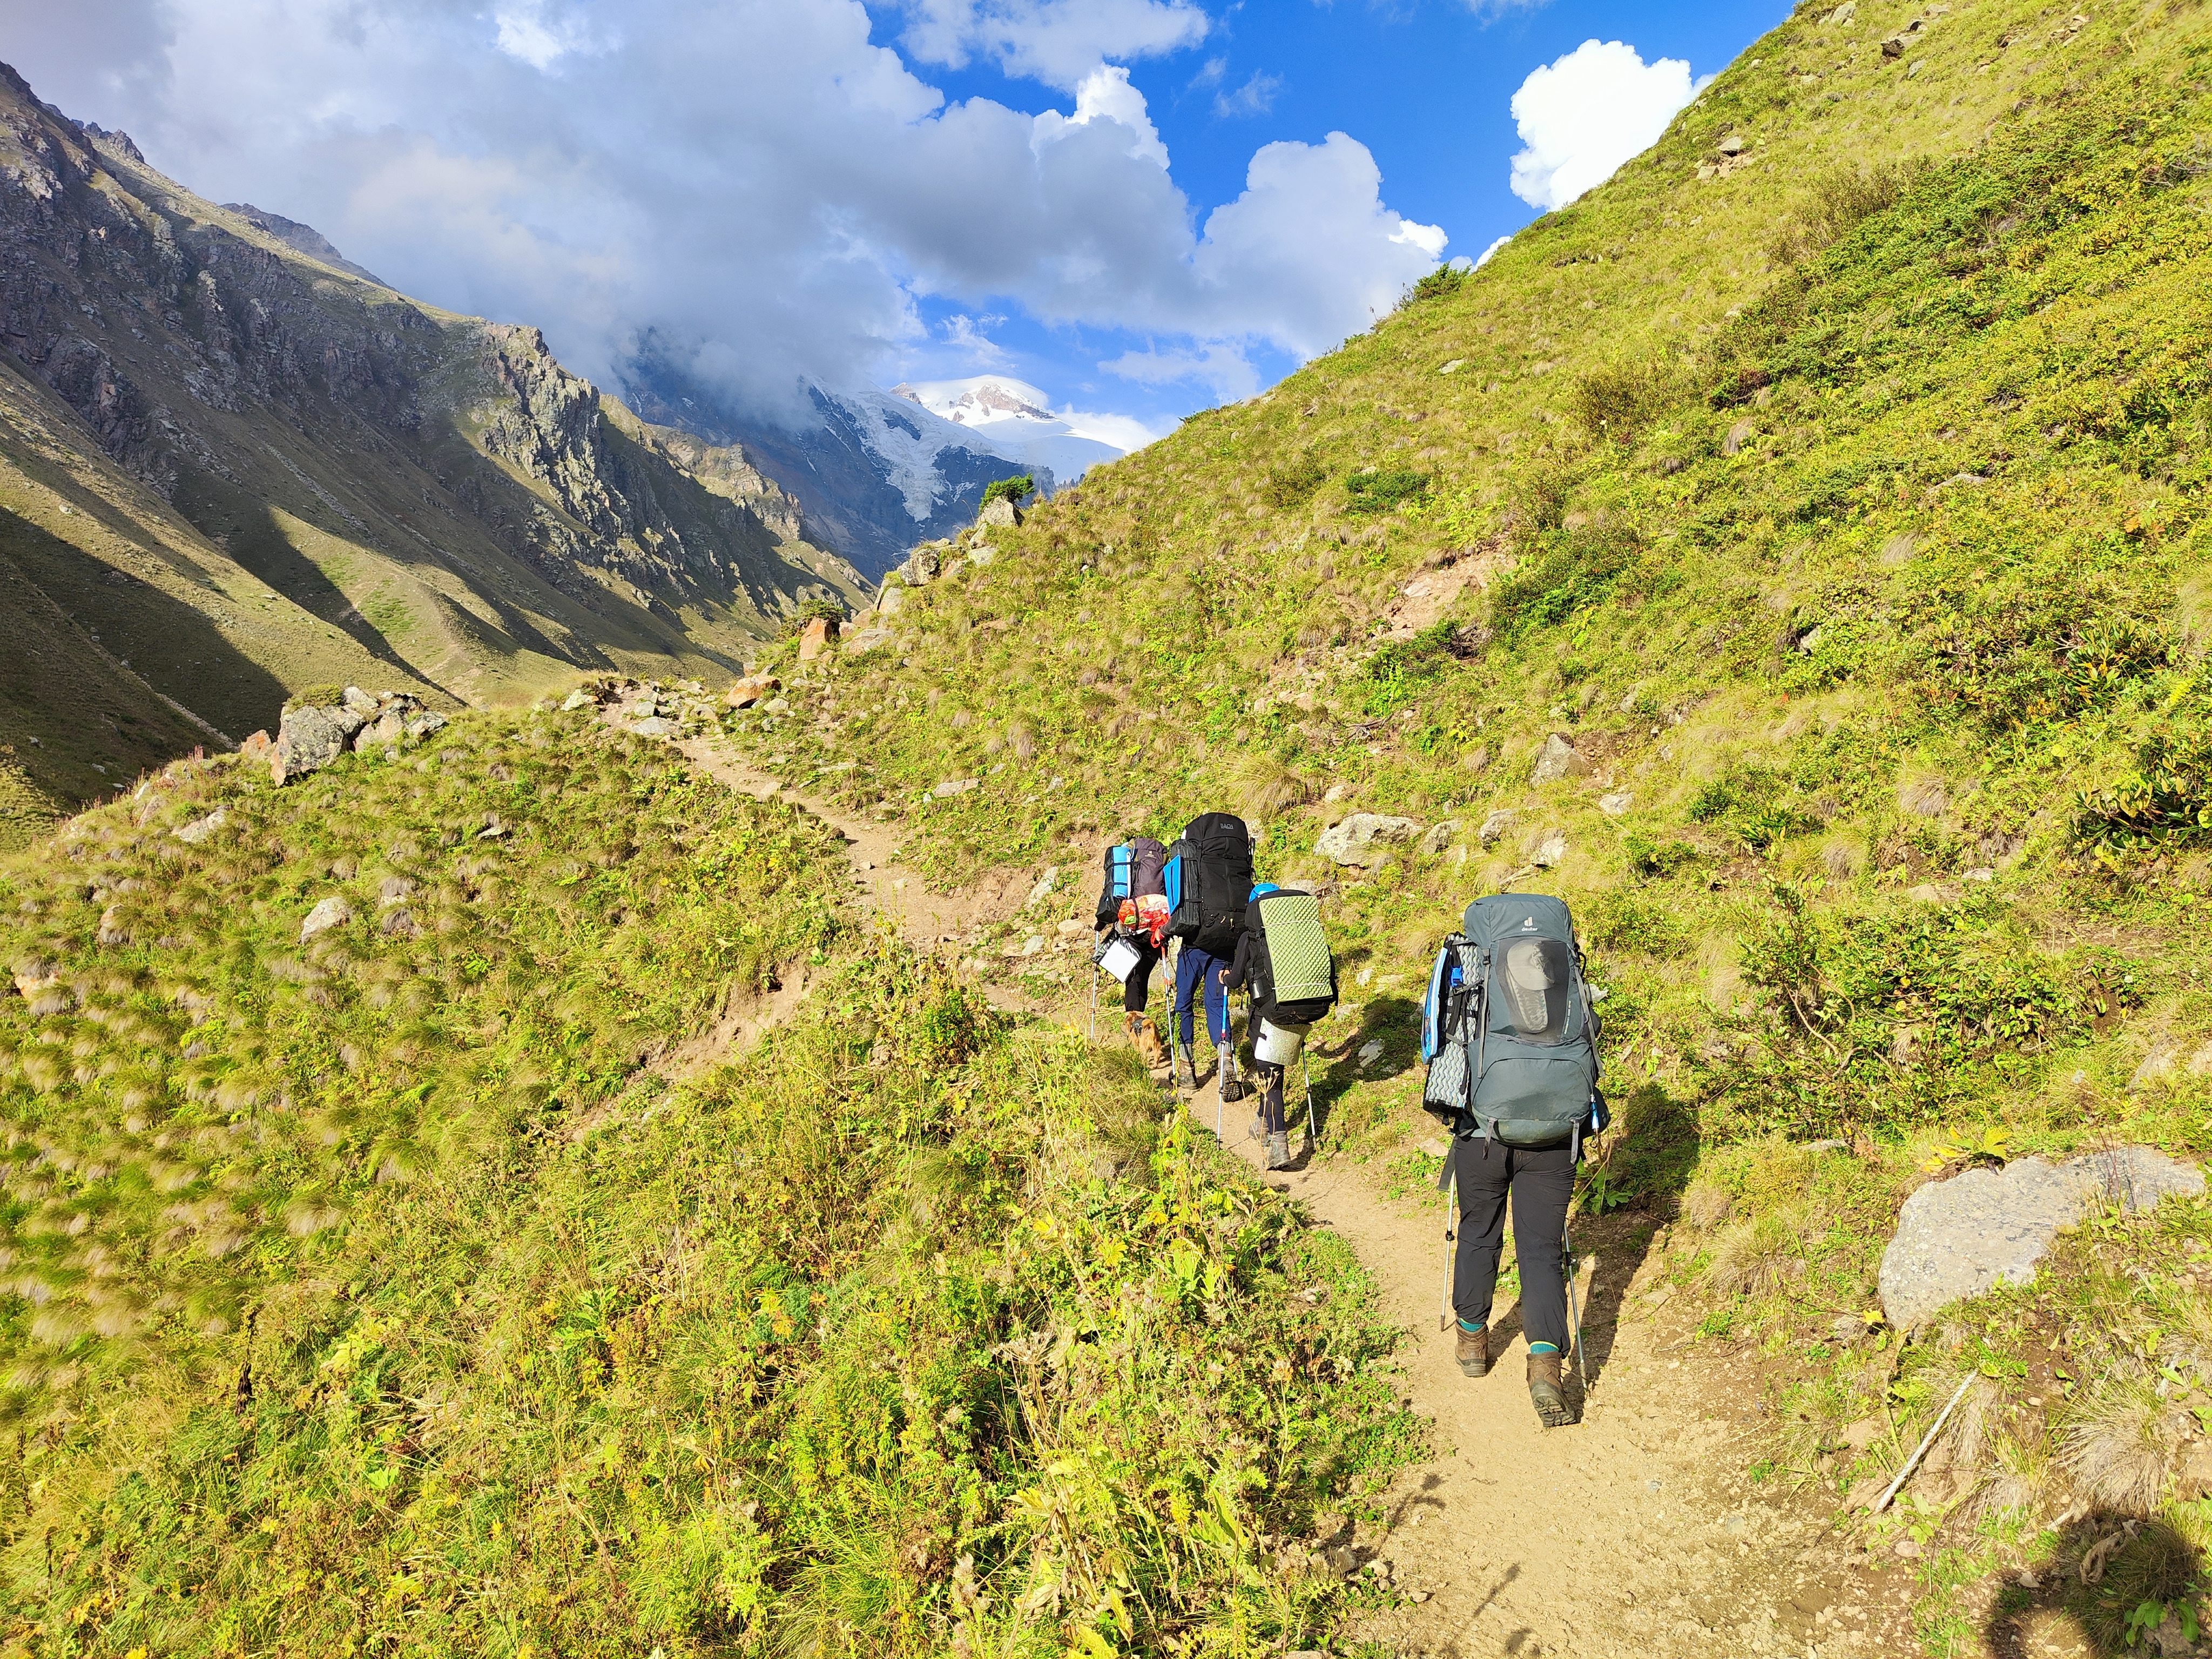
\includegraphics[width=\textwidth]{../pics/IMG_20240829_170756}			
\end{frame}

\begin{frame}
	\frametitle{Вид на Эльбрус с м.н.}
	\framesubtitle{День 12, 29 августа}	
	\centering
	\includegraphics[width=\textwidth]{../pics/IMG_20240829_181353}			
\end{frame}

\begin{frame}
	\frametitle{Место ночёвки 29-30 августа}
	\framesubtitle{День 12, 29 августа}	
	\centering
	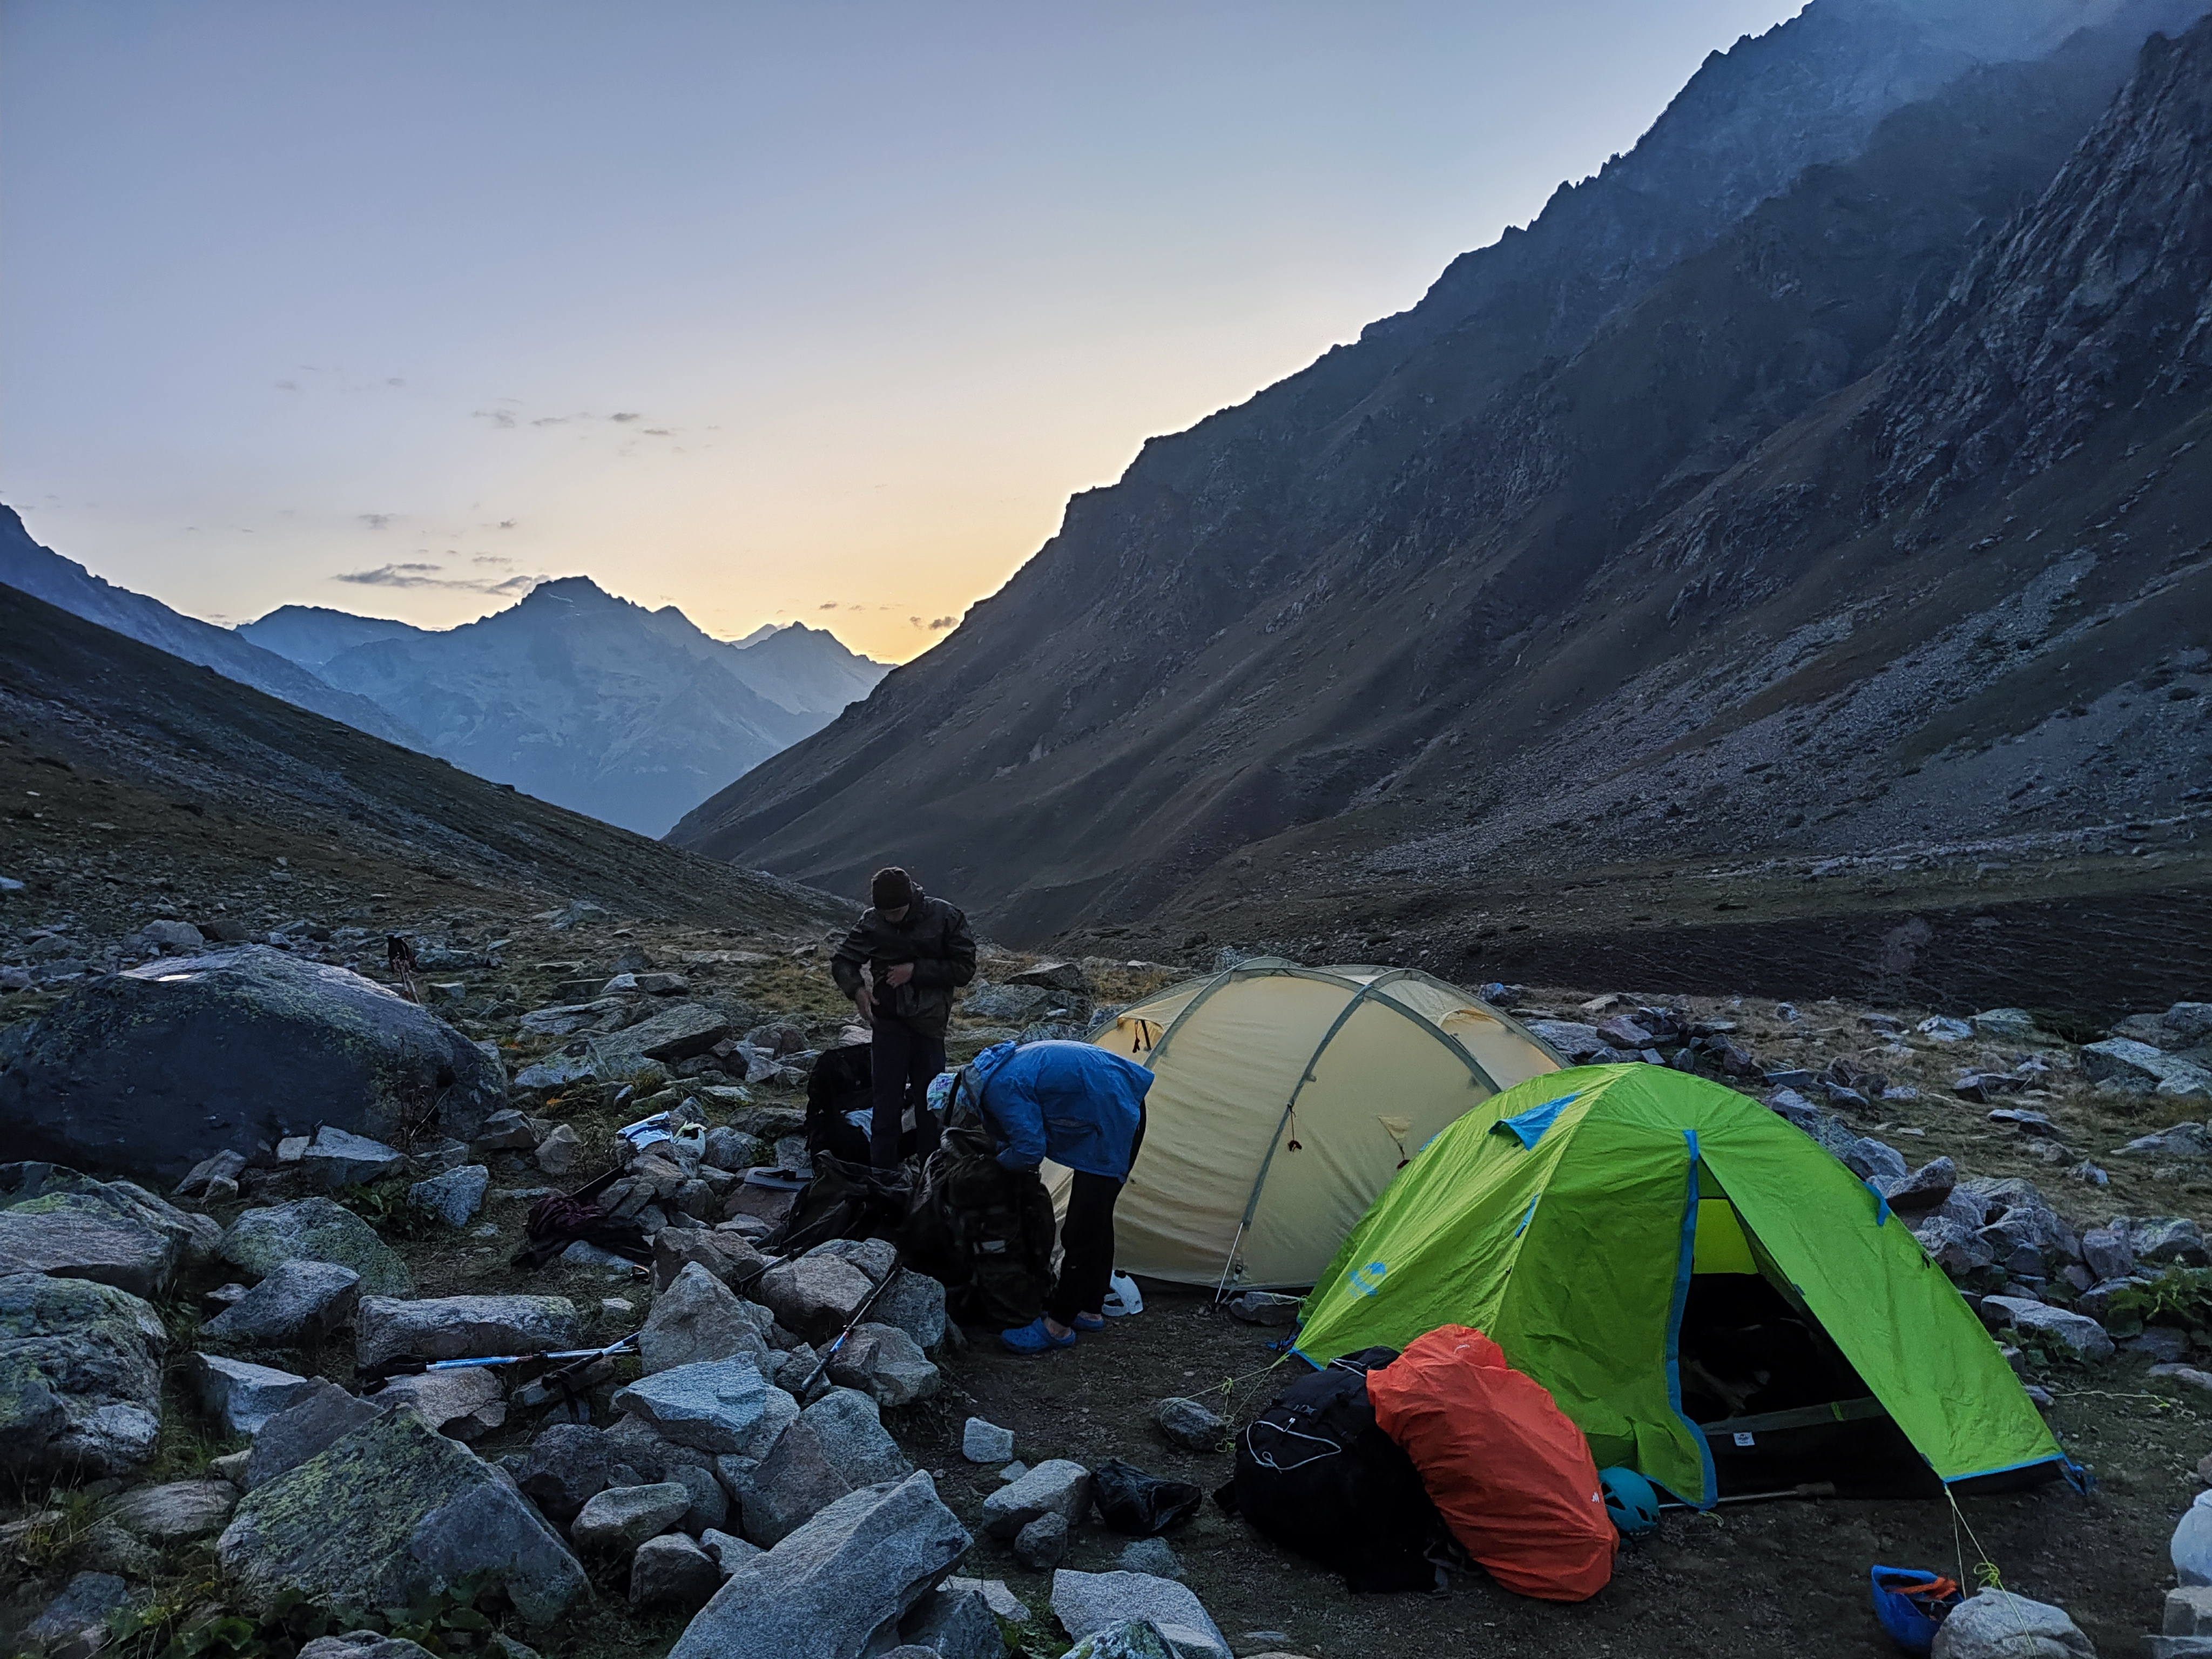
\includegraphics[width=\textwidth]{../pics/IMG_20240829_191225}			
\end{frame}

